\section{Tipos de Cruces} \label{app:crosses}
Tradicionalmente existe cuatro tipos de cruces según su morfología específica básica. Estos cuatro modelos son:
%\begin{itemize}
%\item[La cruz Latina, cruz immissa o cruz ordinaria]
%\item[La cruz Griega o cruz immissa quadrata]
%\item[La cruz de San Andrés o cruz decussata]
%\item[La cruz Tau, cruz commissa o en forma de T]
%\end{itemize}

\begin{description}
\item[] La cruz Latina, cruz \textit{Immissa} o cruz ordinaria
\item[] La cruz Griega o cruz \textit{Immissa quadrata}
\item[] La cruz de San Andrés o cruz \textit{Decussata}
\item[] La cruz Tau, cruz \textit{Commissa} o en forma de T
\end{description}


\begin{figure}[ht!]
    \centering
    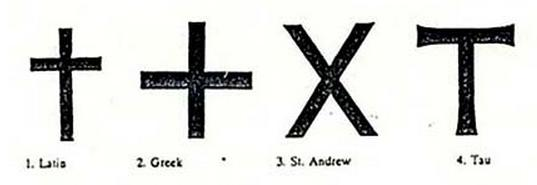
\includegraphics[width=1\textwidth]{cruces.jpg}
    \caption{URL:http://www.crosses.org/history.htm}
\end{figure}